\chapter{Testing Code Area}
%%%%%%%%%%%%%%%%%%%%%%%%%%%%%%%%%%%%%%%%%%%%%%%%%%%%%%%%%%%%%%%%
\begin{table}[H]
	\caption{Caption}
	\label{Label}
	\begin{center}
		\begin{tabular}{||l|l||}\hline
			One & Two \\\hline
			Three & Four \\\hline
		\end{tabular}
	\end{center}
\end{table}
\vspace{1cm}
\begin{figure}[H]
	%%% [H] [ht] [h!]
	%%% \captionsetup{justification=raggedright,singlelinecheck=false}
	%%% \flushleft
	%%% \centering
	%%% \begin{center}
	%%%	\vspace{2.4in}
	%%% \includegraphics[scale=0.52]{./image.jpg}
	%%% \end{center}
	%%% \caption{caption}
	%%% \caption{caption \cite{book_1}}
	%%% \label{label}
\end{figure}
%%%\par
%%%\hspace{1cm}
%%%\clearpage
%%%%%%%%%%%%%%%%%%%%%%%%%%%%%%%%%%%%%%%%%%%%%%%%%%%%%%%%%%%%%%%%
\textcolor{blue}{AZUL}
%%%%%%%%%%%%%%%%%%%%%%%%%%%%%%%%%%%%%%%%%%%%%%%%%%%%%%%%%%%%%%%%
\begin{figure}[H]
	\begin{minipage}{0.3\linewidth}
		\flushleft
		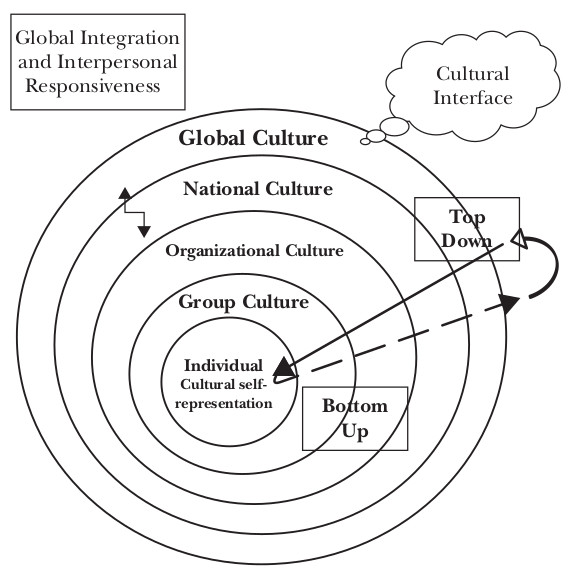
\includegraphics[scale=0.30]{./image/CORGA/OB/OB_MUltilevelmodelCulture.jpg}
	\end{minipage}
	\hspace{1cm}
	\begin{minipage}{0.4\linewidth}
		\flushleft
		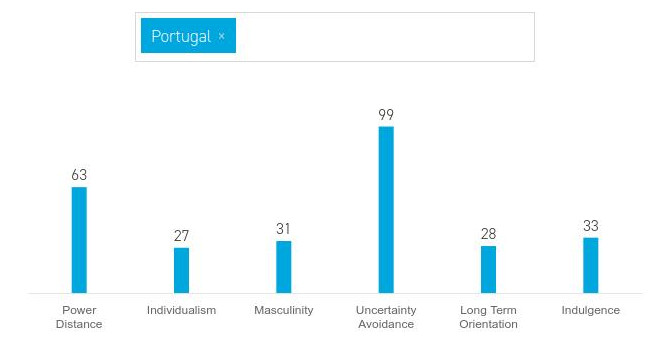
\includegraphics[scale=0.44]{./image/CORGA/OB/Hofstede_pt}
	\end{minipage}
	\caption{Modelo de Multi-níveis \cite{book_11} da cultura e Modelo Hofstede, Portugal}
\end{figure}
%%%%%%%%%%%%%%%%%%%%%%%%%%%%%%%%%%%%%%%%%%%%%%%%%%%%%%%%%%%%%%%%
\begin{itemize}
	\setlength\itemsep{-0.5em}
	\item \textcolor{purple}{Items}
	\begin{itemize}
		\setlength\itemsep{-0.3em}
		\item \textcolor{orange}{Item 1}
		\item \textcolor{orange}{Item 2}
	\end{itemize}
	\item \textcolor{purple}{Items}
	\begin{itemize}
		\setlength\itemsep{-0.3em}
		\item \textcolor{orange}{Item 1}
		\item \textcolor{orange}{Item 2}
	\end{itemize}
\end{itemize}
%%%%%%%%%%%%%%%%%%%%%%%%%%%%%%%%%%%%%%%%%%%%%%%%%%%%%%%%%%%%%%%%
\begin{minipage}[t]{.40\linewidth}
	\quad Estilos de Liderança:
	\begin{itemize}
		\setlength\itemsep{-0.3em}
		\item Participativo
		\item Orientado as pessoas\\
		(Liderança de suporte)
		\item Orientado as tarefas\\
		(Liderança Instrumental\\ ou Diretiva\\ ou Transacional)
	\end{itemize}
\end{minipage}
\begin{minipage}[t]{.30\linewidth}
	\quad Tipos de Cultura:
	\begin{itemize}
		\setlength\itemsep{-0.3em}
		\item Inovadora
		\item Competitiva
		\item Burocrática
		\item Comunitária
	\end{itemize}
\end{minipage}
\begin{minipage}[t]{.40\linewidth}
	\quad Medição do Sucesso:
	\begin{itemize}
		\setlength\itemsep{-0.3em}
		\item Satisfação dos Clientes
		\item Taxa crescimento vendas
		\item Cotação no mercado
		\item Vantagens Competitivas
		\item Volume de vendas
	\end{itemize}
\end{minipage}
\vspace{1cm}
\newline
%%%%%%%%%%%%%%%%%%%%%%%%%%%%%%%%%%%%%%%%%%%%%%%%%%%%%%%%%%%%%%%%
\begin{table}[h!]
	\begin{adjustbox}{max width=\textwidth}
		\begin{tabular}{ |c|l|c| }
			\hline
			\rowcolor[gray]{0.5}
			Nº & Inquérito & \makecell[l]{Resp \\ 1 \; - \; 7} \\
			\hline
			1. & \makecell[l]{A organização preocupa-se com o crescimento e a aquisição de novos recursos, \\ e procura responder a novos desafios.} & \\
			\hline
			2. & \makecell[l]{A organização é dinâmica e empreendedora. \\ As pessoas estão dispostas a correr riscos.} & \\
			\hline
			3. & \makecell[l]{Existe um elevado empenho na inovação e no desenvolvimento. \\ Procuramos ser os primeiros.} & \\
			\hline
			4. & \makecell[l]{Consideram-se os melhores gestores os que são empreendedores, \\ Inovadores e tomadores de riscos.} & \\
			\hline
			5. & Existe uma elevada ênfase nas tarefas e no alcance de objetivos. & \\
			\hline
			6. & Considera-se que os melhores gestores são produtores e técnicos. & \\
			\hline
			7. & \makecell[l]{A organização valoriza as ações competitivas, \\ o sucesso e o alcance de objetivos mensuráveis.} & \\
			\hline
			8. & \makecell[l]{A organização é orientada para a produção. \\ Uma das maiores preocupações é fazer o que tem que ser feito. \\ Os empregados não estão muito envolvidos do ponto de vista pessoal.} & \\
			\hline
			9. & A organização valoriza muito as regras e as políticas formais. & \\
			\hline
			10. & \makecell[l]{A organização é muito formalizada e estruturada. \\ Os procedimentos estabelecidos orientam o que as pessoas devem fazer.} & \\
			\hline
			11. & Os melhores gestores são considerados os que são coordenadores ou organizadores. & \\
			\hline
			12. & Na organização valoriza-se a permanência, a estabilidade e a eficiência. & \\
			\hline
			13. & Valoriza-se muito a lealdade, a tradição e o empenhamento na organização. & \\
			\hline
			14. & A organização é uma espécie de grande família. & \\
			\hline
			15. & Valoriza-se muito a coesão e os recursos humanos. & \\
			\hline
			16. & \makecell[l]{Considera-se que os melhores gestores são os que atuam como mentores, \\ sábios ou figuras paternais/maternais.} & \\
			\hline
		\end{tabular}
	\end{adjustbox}
\end{table}
\vspace{1cm}
\newline
%%%%%%%%%%%%%%%%%%%%%%%%%%%%%%%%%%%%%%%%%%%%%%%%%%%%%%%%%%%%%%%%
\begin{table}[H]
	{\small
		\begin{tabular}{|l|c|c|}
			\hline
			& Média do Inquerito & \begin{tabular}[c]{@{}l@{}}Ogbonna \& Harris\\ (2000)\end{tabular} \\ \hline
			\cellcolor[HTML]{C0C0C0}\begin{tabular}[c]{@{}l@{}}Cultura de inovação\\ {[}1-4{]}\end{tabular}     & 5,4 & 4,6 \cellcolor[HTML]{EFEFEF}                                           \\ \hline
			\cellcolor[HTML]{C0C0C0}\begin{tabular}[c]{@{}l@{}}Cultura de Competição\\ {[}5-8{]}\end{tabular}   & 5,3 & 4,2 \cellcolor[HTML]{EFEFEF}                                           \\ \hline
			\cellcolor[HTML]{C0C0C0}\begin{tabular}[c]{@{}l@{}}Cultura Burocrática\\ {[}9-12{]}\end{tabular}    & 4,7  & 4,3 \cellcolor[HTML]{EFEFEF}                                           \\ \hline
			\cellcolor[HTML]{C0C0C0}\begin{tabular}[c]{@{}l@{}}Cultura de Comunidade\\ {[}13-16{]}\end{tabular} & 5  & 4,6 \cellcolor[HTML]{EFEFEF}                                           \\ \hline
		\end{tabular}
	}
\end{table}
\vspace{1cm}
%%%%%%%%%%%%%%%%%%%%%%%%%%%%%%%%%%%%%%%%%%%%%%%%%%%%%%%%%%%%%%%%
\hspace*{5cm} - HSPACE 5cm
\newline
\vspace{1cm}
\newline
%%%%%%%%%%%%%%%%%%%%%%%%%%%%%%%%%%%%%%%%%%%%%%%%%%%%%%%%%%%%%%%%
\begin{minipage}{.75\linewidth}
	\begin{tabular}{ |c|c|c|c|c|c|c|c|c|c|c|c| }
		\hline
		\rowcolor[gray]{0.7}
		$h_i$ & CLASSE & MARCA & $n_{i_A}$ & $n_{i_B}$ & $\frac{n_{i_A}}{h_i}$ & $\frac{n_{i_B}}{h_i}$ & $f_{i_A}$	& $f_{i_B}$ & $F_{i_A}$ & $F_{i_B}$ & $e_{i_A}$ \\
		\hline
		$-\infty$ & < 5 & & 0 & 0 & & & & & & & \textcolor{yellow}{1,1812} \\
		\hline
		4 & [5,10[ & 7,5 & 8 & 1 & 2 & 0,25 & 0,0667 & 0,0083 & 0,0667 & 0,0083 & \textcolor{yellow}{5,9871}\\
		\hline
		4 & [10,15[ & 12,5 & 16 & 18 & 4 & 4,5 & 0,1333 & 0,15 & 0,2 & 0,1583 & 18,8942\\
		\hline
		4 & [15,20[ & 17,5 & 40 & 28 & 10 & 7 & 0,3333 & 0,2333 & 0,5333 & 0,3917 & 33,6282\\
		\hline
		4 & [20,25[ & 22,5 & 25 & 41 & 6,25 & 10,25 & 0,2083 & 0,3417 & 0,7417 & 0,7333 & 33,7887\\
		\hline
		4 & [25,30[ & 27,5 & 26 & 22 & 6,5 & 5,5 & 0,2167 & 0,1833 & 0,9583 & 0,9167 & 19,1663\\
		\hline
		4 & [30,35[ & 32,5 & 4 & 8 & 1 & 2 & 0,0333 & 0,0667 & 0,9917 & 0,9833 & \textcolor{orange}{6,1316}\\
		\hline
		5 & [35,40] & 37,5 & 1 & 2 & 0,2 & 0,4 & 0,0083 & 0,0167 & 1 & 1 & \textcolor{orange}{1,1044}\\
		\hline
		$+\infty$ & >40 & & 0 & 0 & & & & & & & \textcolor{orange}{0,1183}\\
		\hline
		& & & n=120 & n=120 & & & & & & & \\
		\hline
	\end{tabular}
\end{minipage}
\vspace{1cm}
\newline
%%%%%%%%%%%%%%%%%%%%%%%%%%%%%%%%%%%%%%%%%%%%%%%%%%%%%%%%%%%%%%%%
\begin{minipage}[!b]{0.40\linewidth}
	\begin{tabular}{ l c c }
		\hline
		Estatística & $X_A$ & $X_B$ \\
		\hline
		Mínimo & 7,5 & 7,5\\
		$Q_1$:$1^o$ Quartil & 17,5 & 17,5 \\
		$m_d$: mediana & 17,5 & 22,5\\
		$Q_3$:$3^o$ Quartil & 27,5 & 27,5 \\
		Máximo & 37,5 & 37,5 \\
		\hline
		$\bar{X}$ : Média & 20,0417 & 21,5417 \\
		$s$ : desvio-padrão & 6,4494 & 6,0909\\
		$m_o$: moda & 17,5 & 22,5\\
		\hline
		Tamanho amostral [$n$] & 120 & 120 \\
		\hline
	\end{tabular}
	\label{Tab:Resultados}
\end{minipage}
\hspace{2cm}
%%%%%%%%%%%%%%%%%%%%%%%%%%%%%%%%%%%%%%%%%%%%%%%%%%%%%%%%%%%%%%%%
\begin{minipage}[!b]{0.40\linewidth}
	\begin{figure}[H]
		\centering
		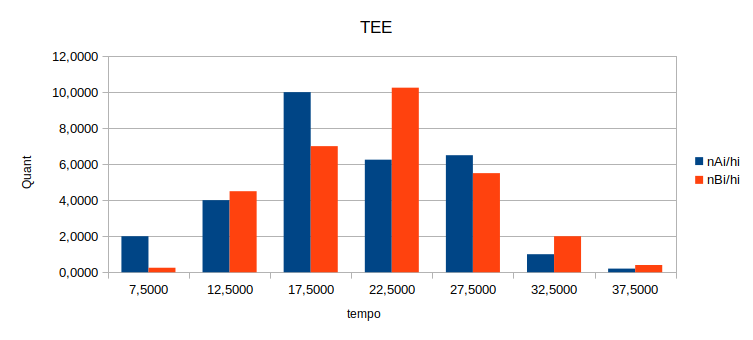
\includegraphics[scale=0.5]{./image/ESTAT/TEE.png}
		\caption{TEE}
		\label{TEE}
	\end{figure}
\end{minipage}
\newline
\vspace{1cm}
\newline
%%%%%%%%%%%%%%%%%%%%%%%%%%%%%%%%%%%%%%%%%%%%%%%%%%%%%%%%%%%%%%%%
\begin{minipage}[!b]{0.45\linewidth}
	\begin{figure}[H]
		\centering
		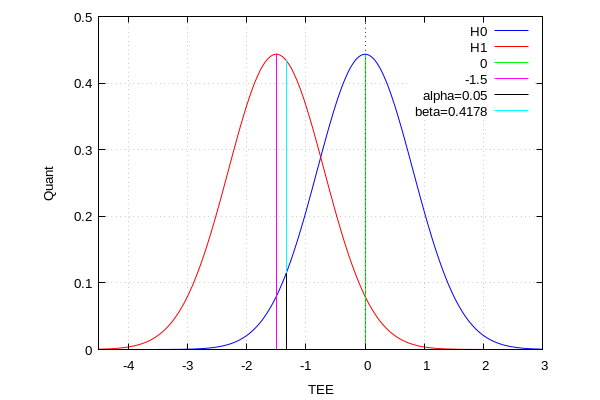
\includegraphics[scale=0.4]{./image/ESTAT/TEE_DIFF.png}
		\caption{TEE Diferênça}
		\label{TEEDIFF}
	\end{figure}
\end{minipage}
\hspace{1cm}
\begin{minipage}[!b]{0.45\linewidth}
	\begin{figure}[H]
		\centering
		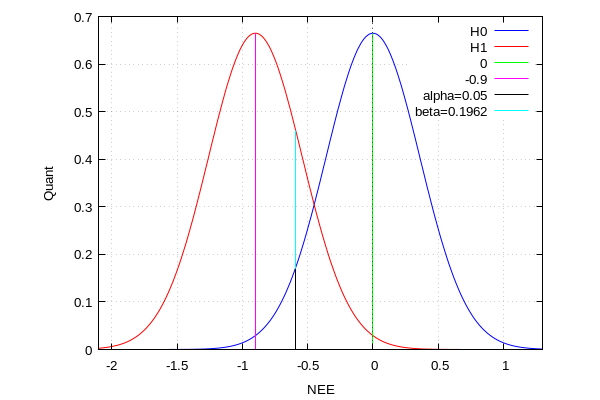
\includegraphics[scale=0.4]{./image/ESTAT/NEE_DIFF.png}
		\caption{NEE Diferença}
		\label{NEEDIFF}
	\end{figure}
\end{minipage}
\newline
\begin{minipage}[!b]{0.45\linewidth}
	\begin{figure}[H]
		\centering
		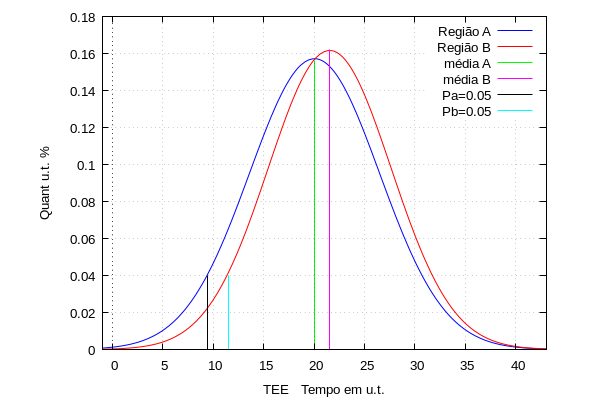
\includegraphics[scale=0.4]{./image/ESTAT/TEE_NORM_DIST.png}
		\caption{TEE Normal}
		\label{TEENORM}
	\end{figure}
\end{minipage}
\hspace{1cm}
\begin{minipage}[!b]{0.45\linewidth}
	\begin{figure}[H]
		\centering
		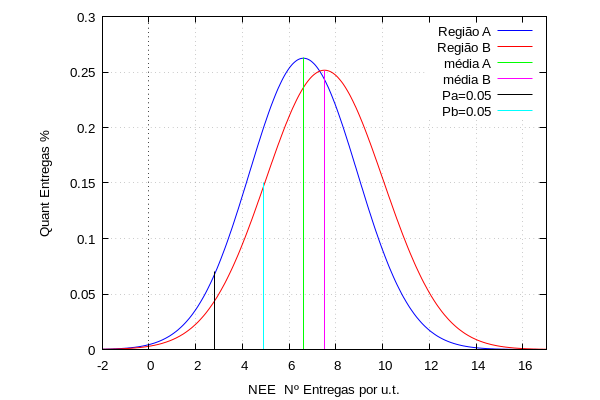
\includegraphics[scale=0.4]{./image/ESTAT/NEE_NORM_DIST.png}
		\caption{NEE Normal}
		\label{NEENORM}
	\end{figure}
\end{minipage}
\newline
\begin{minipage}[!b]{0.45\linewidth}
	\begin{figure}[H]
		\centering
		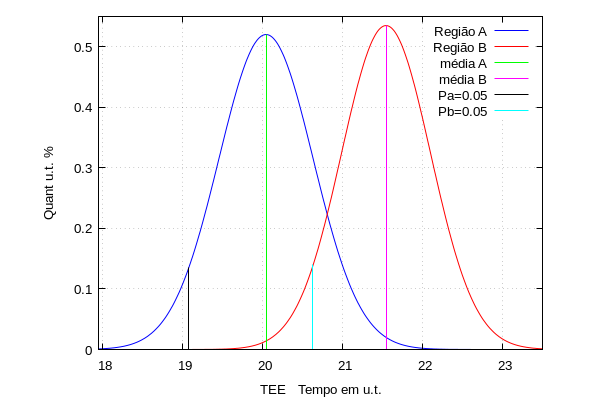
\includegraphics[scale=0.4]{./image/ESTAT/TEE_MEDIA_DIST.png}
		\caption{TEE Normal Média}
		\label{TEEMED}
	\end{figure}
\end{minipage}
\hspace{1cm}
\begin{minipage}[!b]{0.45\linewidth}
	\begin{figure}[H]
		\centering
		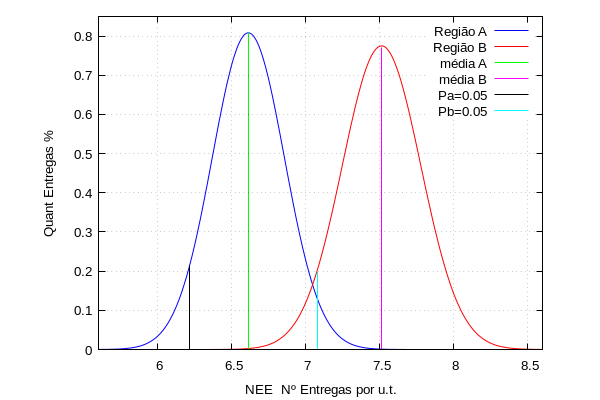
\includegraphics[scale=0.4]{./image/ESTAT/NEE_MEDIA_DIST.png}
		\caption{NEE Normal Média}
		\label{NEEMED}
	\end{figure}
\end{minipage} \\
%%%%%%%%%%%%%%%%%%%%%%%%%%%%%%%%%%%%%%%%%%%%%%%%%%%%%%%%%%%%%%%%
%%%%%%%%%%%%%%%%%%%%%%%%%%%%%%%%%%%%%%%%%%%%%%%%%%%%%%%%%%%%%%%%
%%%%%%%%%%%%%%%%%%%%%%%%%%%%%%%%%%%%%%%%%%%%%%%%%%%%%%%%%%%%%%%%
%%%%%%%%%%%%%%%%%%%%%%%%%%%%%%%%%%%%%%%%%%%%%%%%%%%%%%%%%%%%%%%%
%%%%%%%%%%%%%%%%%%%%%%%%%%%%%%%%%%%%%%%%%%%%%%%%%%%%%%%%%%%%%%%%
%%%%%%%%%%%%%%%%%%%%%%%%%%%%%%%%%%%%%%%%%%%%%%%%%%%%%%%%%%%%%%%%
%%%%%%%%%%%%%%%%%%%%%%%%%%%%%%%%%%%%%%%%%%%%%%%%%%%%%%%%%%%%%%%%
%%%%%%%%%%%%%%%%%%%%%%%%%%%%%%%%%%%%%%%%%%%%%%%%%%%%%%%%%%%%%%%%
%%%%%%%%%%%%%%%%%%%%%%%%%%%%%%%%%%%%%%%%%%%%%%%%%%%%%%%%%%%%%%%%
%%%%%%%%%%%%%%%%%%%%%%%%%%%%%%%%%%%%%%%%%%%%%%%%%%%%%%%%%%%%%%%%
%%%%%%%%%%%%%%%%%%%%%%%%%%%%%%%%%%%%%%%%%%%%%%%%%%%%%%%%%%%%%%%%
%%%%%%%%%%%%%%%%%%%%%%%%%%%%%%%%%%%%%%%%%%%%%%%%%%%%%%%%%%%%%%%%
%%%%%%%%%%%%%%%%%%%%%%%%%%%%%%%%%%%%%%%%%%%%%%%%%%%%%%%%%%%%%%%%
%%%%%%%%%%%%%%%%%%%%%%%%%%%%%%%%%%%%%%%%%%%%%%%%%%%%%%%%%%%%%%%%
\begin{comment}
%%%%%%%%%%%%%%%%%%%%%%%%%%%%%%%%%%%%%%%%%%%%%%%%%%%%%%%%%%%%%%%%
Característica de bons Objetivos\\
- Claros\\
- Concisos\\
- Calendarizados\\
- Atingíveis\\
%%%%%%%%%%%%%%%%%%%%%%%%%
Tipos de organizações\
- Organização privadas com fins lucrativos\\
- Organização privadas sem fins lucrativos\\
- Organização publicas com fins lucrativos\\
- Organização publicas sem fins lucrativos\\
%%%%%%%%%%%%%%%%%%%%%%%%%
tipos de hierarquias\\
tipos de departamentalizações\\
organização por processo\\
%%%%%%%%%%%%%%%%%%%%%%%%%
A divisão do trabalho, permitiu a redução do tempo de aprendizagem, isto é, cada um tem as suas funções, aumentando a produtividade. Cada um executa uma parte das tarefas necessárias a fabricação.\\
%%%%%%%%%%%%%%%%%%%%%%%%%
Gestão:\\ \\
\begin{minipage}{20cm}
\begin{minipage}{5cm}
Instrumentos
\begin{enumerate}
\item Planear
\item Organizar
\item Controlar\\ \\
\end{enumerate}
\end{minipage}
\begin{minipage}{5cm}
Funções
\begin{enumerate}
\item Liderança
\item Comunicação
\item Motivação
\item Tomada de decisão
\end{enumerate}
\end{minipage}
\end{minipage}
%%%%%%%%%%%%%%%%%%%%%%%%%
Cadeia de valor\\
-Atividades principais\\
-Atividades de suporte\\
%%%%%%%%%%%%%%%%%%%%%%%%%
\end{comment}
%%%%%%%%%%%%%%%%%%%%%%%%%%%%%%%%%%%%%%%%%%%%%%%%%%%%%%%%%%%%%%%%
%%%%%%%%%%%%%%%%%%%%%%%%%%%%%%%%%%%%%%%%%%%%%%%%%%%%%%%%%%%%%%%%
%%%%%%%%%%%%%%%%%%%%%%%%%%%%%%%%%%%%%%%%%%%%%%%%%%%%%%%%%%%%%%%%
